\section{SONAR Classification 101 and MACS Workflow}

\subsection{What you will learn in this section}

\begin{compactenum}
    \item How to understand and use LOFAR and DEMON.
    \item How calculate propeller shaft and blade rates (SR BR) to provide signature information and an estimate of the vessels speed.
    \item Understand what the different diesel engine configurations are including calculating Individual Cylinder Firing Rate (ICFR), Crankshaft Rate (CSR), Engine Firing Rate (EFR) and determining the number of cylinders.
    \item How to recognise harmonics, sidebands and reduction ratios and understand how a contact can be classified from these signatures.
    \item How to recognise additional information and distinguish if these signatures are engine or shaft related, or are fixed features such as electrical mains.
\end{compactenum}

\textbf{Before attempting the examples in Section 7, you should read and have a reasonable grasp of this section.}

\begin{faintquote}
    This section introduces some of the basic mathematics behind SONAR analysis all of which is simple arithmetic and can be done with a calculator. The deep mathematics behind Fourier Transforms and cepstrum analysis is more complicated but you do not need knowledge at that level to enjoy MNW or use MACS. For those interested in the deeper detail you will find it in Appendix B.
\end{faintquote}

Although it is tempting to dive in to the powerful tools available in MACS you should, at first, take a step back as a useful amount of data can be collected by simply listening. After an initial assessment you will be working primarily with the MACS LOFAR and DEMON screens. If these are new names for you, read Section 2 \textbf{SONAR and Sound Analysis an Introduction}. You may also use the CEPSTRUM and Auto-Correlation (ACF) features explained below and in Appendix B. 

A LOFARgram is a visual representation of the LOFAR analysis, it is generally not something an inexperienced user can interpret just by looking at it. Sonar analysts are not simply spotting lines, they are using their knowledge of how machinery generates frequencies, how they relate mathematically to one another and to specific machinery. When you are trying to understand what you are hearing think of yourself as a detective. Observe patterns, form hypotheses, test them mathematically and look for evidence that supports or disproves them.

\begin{faintquote}
    As with any good hypothesis the best is usually the one that explains the greatest number of outcomes with the fewest assumptions (Occam).
\end{faintquote}

The LOFARgram is your primary tool. The display is a waterfall of the sound spectrum, with brightness indicating signal strength. In MACS, time flows from bottom to top and frequency runs left to right on the horizontal (\textit{x}) axis; often called the frequency domain.

You are looking for: \textbf{Tonals (narrowband lines)} These appear as bright \textbf{vertical lines}, a continuous stripe at a fixed frequency persisting as time scrolls past. Every significant machine on a vessel produces a characteristic set of tonals: main engine, generators, pumps, turbines. Although, they may not always be visible. The most common cause of poor broadband resolution is poor signal to noise ratio and orientation to the target. The LAB has a blind spot directly astern and the towed arrays have blind spots directly ahead.

The DEMON display is your primary analysis tool for \textbf{propeller configuration and SR.} When a marine vessel travels through water, the rotating propeller blades can create pockets of low pressure forming tiny vapour bubbles that rapidly collapse; a phenomenon known as cavitation. This collapse produces a continuous, broadband hissing noise. As the propeller rotates it causes an amplitude modulation at lower frequencies corresponding directly to the physical movement of the mechanical propulsion system. Essentially, the high-frequency cavitation acts as a "carrier wave" that is amplitude modulated (AM) by the low-frequency mechanics of the ship.

However even without cavitation, the propeller/ship can produce broadband noise whose amplitude varies periodically with shaft or blade rotation. The following lists some of these other sources.

\begin{compactitem}
    \item Non-uniform wake into the propeller. Water reaching the propeller is not uniform because the hull, appendages and shafting disturb the flow. As each blade rotates through regions of faster/slower or more turbulent inflow, its hydrodynamic loading changes. That can modulate the radiated noise at blade rate and harmonics.
    \item Blade-to-blade differences. Real propellers are not perfectly identical. Small differences in blade geometry, fouling, damage or loading can make one blade noisier than another. That can introduce modulation at shaft rate, because that distinctive blade comes round once per revolution.
    \item Turbulent boundary-layer/wake noise. Even without vapour cavitation, turbulent water interacting with the propeller and hull produces broadband pressure fluctuations. Rotation through a non-uniform turbulent field can impose periodic structure on that otherwise random broadband noise.
    \item Propeller/hull interaction. The periodically varying forces generated by the rotating propeller can interact with the stern/hull and radiate noise. This can contain shaft-rate and blade-rate periodicities.
    \item Rotating machinery. Pumps, motors, gears, bearings and other machinery can generate broadband vibration/noise whose level is periodically modulated by rotation. This isn't necessarily propeller -DEMON, but mathematically DEMON-type envelope analysis can reveal those periodicities too.
\end{compactitem}

The resulting output, often displayed as a DEMONgram, reveals distinct spectra that correspond to the vessel's unique physical traits. Sonar operators analyze these lines to identify important features of the  target. By revealing these mechanical design characteristics, the specific class, or even the individual identity, of a target submarine or surface ship can be determined with a good degree of confidence.

\begin{faintquote}
    The transition from “finding lines” to “recognising families, harmonics, and sidebands” is usually the point where a trainee starts thinking like an analyst rather than an operator.
\end{faintquote} 

The ultimate aim of a SONAR analysis is to create a "fingerprint" of the vessel under consideration. It is not necessarily to categorically identify an individual ship, although than can happen. Instead the information derived is stored in a database. This data can then be used to match future encounters and narrow down the type and classification of vessels. Over time more detail can be added refining the classification. The key diagnostic information usually sought includes:

\begin{compactitem}
    \item Engine types (diesel, turbine, electric drive)
    \item Ship propulsion fundamentals (BR, SR)
    \item Number of prepeller shafts
    \item Propeller blade counts
    \item Engine characteristics (CSR, Number of cylinders, EFR and ICFR)
    \item Gear Mesh Frequency (GMF), Gearbox arrangements and reduction ratios
    \item Electrical mains frequencies
\end{compactitem}

First though we need to understand a couple of important terms.

\subsection{What are Harmonics?}

Harmonics occur because real machinery does not produce perfectly smooth vibrations. A perfect rotating shaft would generate a pure tone at one frequency (sinusoidal) but real machinery isn't perfect it produces pulses, impacts, and uneven forces (Figure 13). Diesel engines don't apply torque smoothly, each combustion event is a pulse. A 15 Hz engine-related frequency might produce harmonics at 15, 30, 45, 60 and 75 Hz. Harmonics are always a fixed distance apart and always an integer multiplication of the fundamental, in this case 15 Hz multiplied by 2, 3, 4 etc. SONAR analysts love harmonics because whilst a single line on a LOFARgram is weak evidence, a harmonic family is powerful evidence. Sometimes the fundamental line may not be visible but can be inferred by back-counting the harmonics. MACS provides tools to do this automatically and to confirm the periodicity of suspected harmonics. The sources of the variation could be one or more of:

\begin{compactitem} 
    \item Uneven forces
    \item Multiple cylinders
    \item Gear teeth impacts
    \item Bearing imperfections
    \item Structural resonances
    \item Blade loading variations
\end{compactitem}

\begin{faintquote}
    \textbf{Why is this important}: because in our diesel engine the harmonics point back to the fundamental value (15 Hz). Even if the fundamental is weak, the harmonics may reveal it.
\end{faintquote}


\begin{figure}[ht]
	\centering
	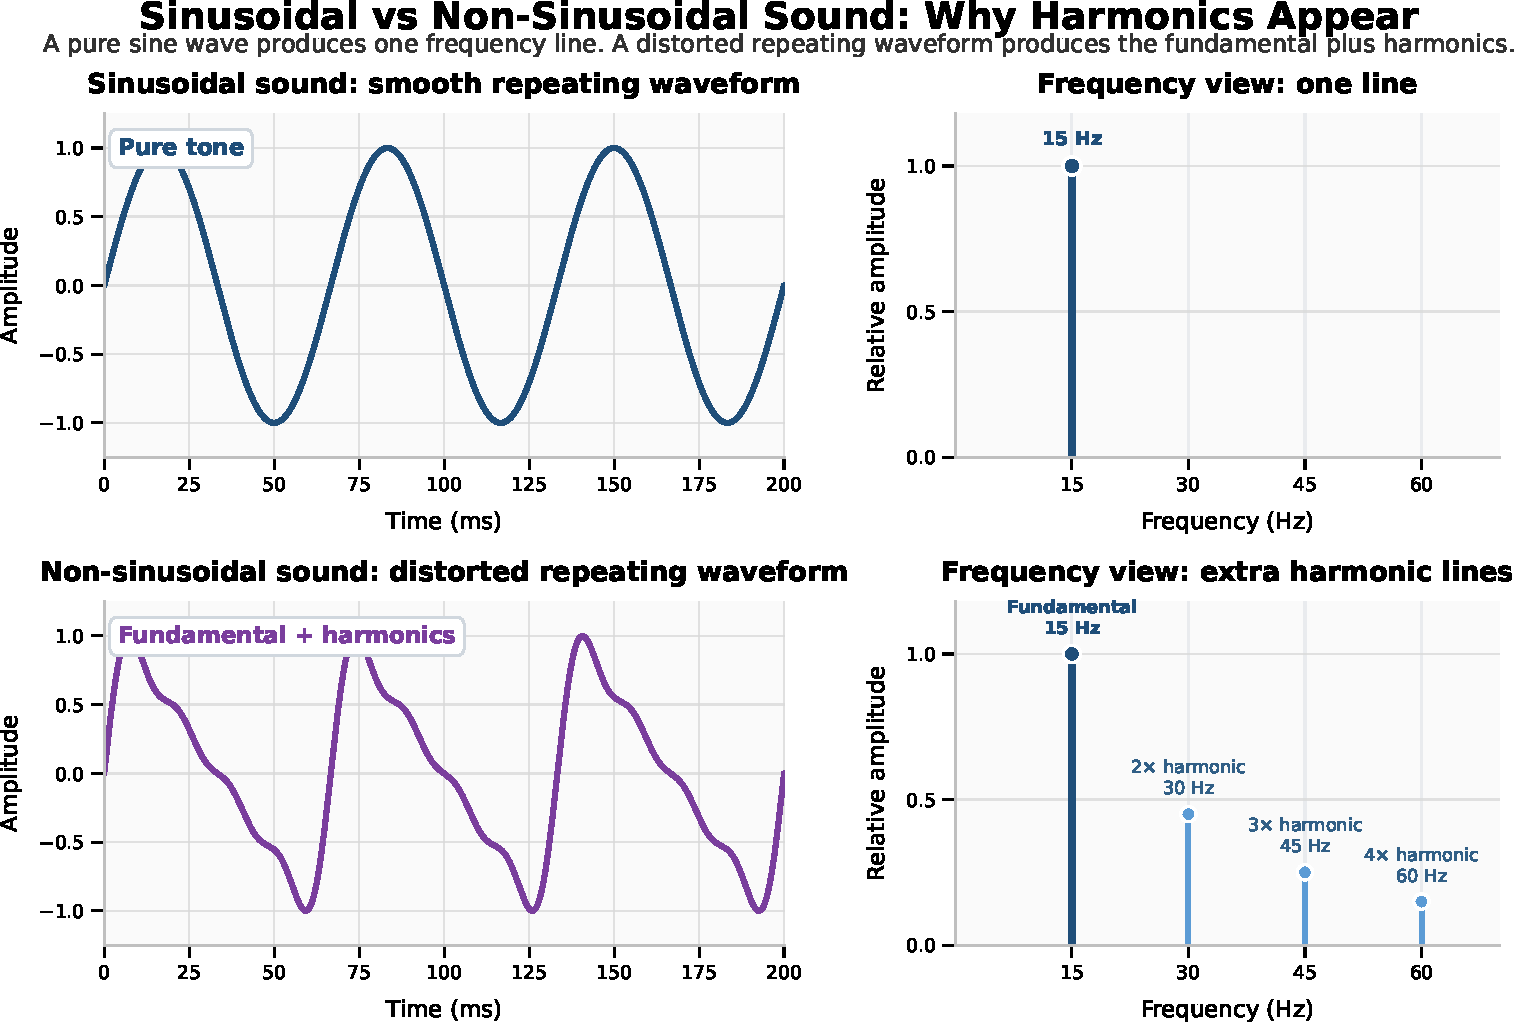
\includegraphics[width=\textwidth]{../img/actuals/sinusoidal_vs_nonsinusoidal_sound.pdf}
	\caption{Harmonics caused by sinusoidal waveform vs non-sinusoidal waveform}
\end{figure}

\subsection{What are Sidebands?}

In radio, a carrier frequency is modified by amplitude (AM) or frequency (FM), the carrier doesn't disappear, instead, additional frequencies appear on either side of it. The same occurs with machinery. An AM sideband, caused by a damaged bearing clicking once per revolution, creates a periodic rise and fall in the amplitude of the high-frequency machinery noise. AM produces exactly one pair of symmetrical sidebands $(f_c + f_m \mathrm{ \ and\ } f_c - f_m)$. In FM modulation the frequency is shifted up and down. A rotating propeller shaft might vibrate causing the carrier frequency to speed up or slow down. FM produces an infinite series of sidebands (Figure 14 Page 24) spaced at intervals of $f_m \quad (f_c \pm f_m, f_c \pm 2f_m, f_c \pm 3f_m ...)$. Suppose a gearbox produces a strong tone at 150 Hz and a propeller shaft rotates at 2.5 Hz. If the shaft causes the gearbox load to increase and decrease once per revolution, the 150 Hz gear tone is being modulated at 2.5 Hz. Instead of 150 Hz you get 145, 147.5, 150, 152.5 and 155 Hz.

In reality, targets rarely exhibit pure AM or pure FM. A propeller blade passing close to a ship's hull undergoes dynamic pressure changes simultaneously altering the amplitude of the acoustic wave (AM) and slightly shifting the phase/frequency (FM). Sonar analysts use specialized tools like DEMON processing to isolate these combined sidebands and identify the specific machinery signatures of a vessel.

\textbf{Sideband Recognition Rule:} when you spot a strong tonal:

\begin{compactenum}
    \item Find the centre frequency.
    \item Look equally above and below it. Is it symmetrical?
    \item Measure the spacing.
    \item Check whether the same spacing exists elsewhere.
    \item Look to see if the lines move together as the target vessel's speed changes
    \item Hypothesise: "Could this spacing be a shaft rate, blade rate, or engine-related rate?"
\end{compactenum}

\begin{figure}[ht]
	\centering
	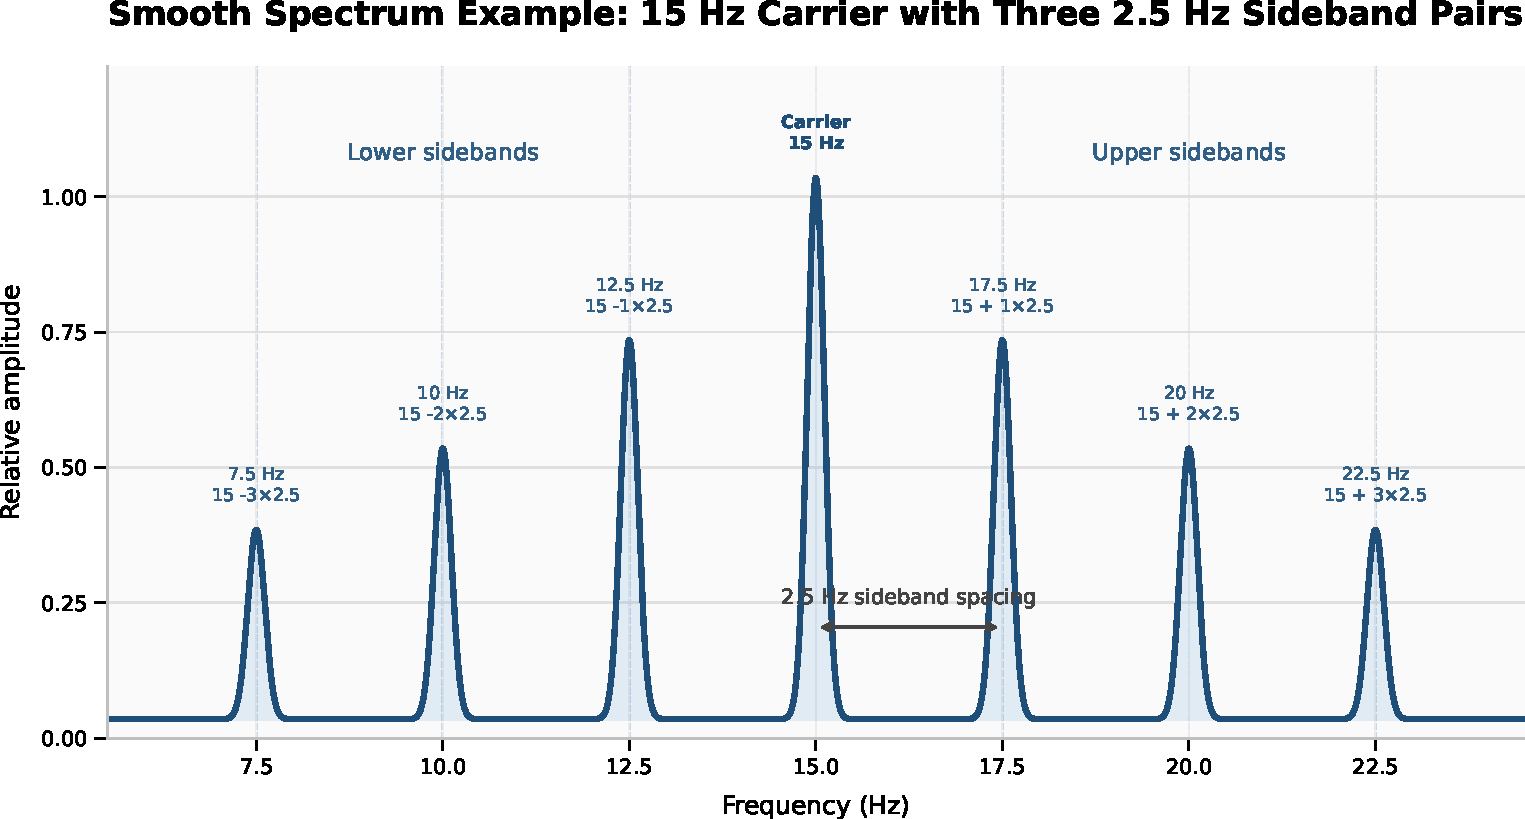
\includegraphics[width=\textwidth]{../img/actuals/sideband.pdf}
	\caption{Sidebands caused by modulation}
\end{figure}

\begin{faintquote}
    The sideband spacing is often the real clue frequently telling you more about the machinery than the large central line itself.
\end{faintquote}

\subsection{LOFARgrams - what to look for}

\begin{compactitem}
    \item \textbf{Fundamental engine frequencies} and their harmonics e.g. CSR, EFR and gear mesh.
    \item \textbf{Blade rate} = $SR \times BC$. May be visible in the 5 - 100 Hz range for surface ships although low frequency tonals are more likely to be spotted in DEMON.
    \item \textbf{Electrical mains} typically multiples of 50 or 60 Hz.
    \item \textbf{Generator harmonics} The GenSet is often an independent motor with its own rotating components producing tonals specific to it.
    \item \textbf{Broadband noise level} A vessel moving fast will show a raised broadband floor (cavitation); the entire display is brighter. A slow or quiet vessel may show almost no broadband increase, with only discrete tonals against a dark background.
    \item \textbf{Frequency drift} A tonal that slowly shifts upward or downward in frequency is Doppler-shifted, meaning the contact's radial velocity (range rate) is changing. It is accelerating, decelerating, or turning. A line that stays at a fixed frequency means the radial velocity is constant, but this says nothing about absolute range; the contact could be closing, opening, or crossing at a steady speed.
\end{compactitem}

\textbf{Practical tips:}
\begin{compactitem}
    \item Zoom Fmin / Fmax around a suspected harmonic family to check spacing.
    \item Enable normalisation to make weak tonals visible against a noisy floor.
    \item Use noise reference subtraction if own-ship noise is masking the target.
    \item Use harmonic cursor mode to check whether a candidate fundamental has a regular harmonic family above it.
\end{compactitem}

\subsection{DEMONgrams - what to look for}

\begin{compactitem}
    \item \textbf{Shaft rate (SR) for propeller-driven vessels:} The most prominent peak in the DEMON output is typically the shaft fundamental. A shaft rotating at 5 Hz will show a strong peak at 5 Hz in the DEMON waterfall.
    \item \textbf{Blade count (BC) for propeller driven vessels:} The number of blades on the propeller(s).
    \item \textbf{Blade rate (BR)} can be calculated with $SR \times BC$ e.g. if the shaft is at 5 Hz and the vessel has 5 blades, the blade rate is 25 Hz, look for a peak there.
    \item \textbf{Engine Firing Rate (EFR):} Diesel or diesel-electric engines produce strong modulation at the crankshaft rate (CSR) and its harmonics. See sub-section 6.10 for method.
    \item \textbf{Harmonic series:} Both shaft and engine signals produce harmonic combs at fundamental, 2x, 3x. Look for evenly spaced peaks using the harmonic cursor mode to confirm the family.
\end{compactitem}

\textbf{Practical tips:}

\begin{compactitem}
    \item Set Band band of strong broadband noise for best signal to noise ratio (SNR) see table below.
    \item Set $F_{max}$ to a value which maximises the coverage of the frequency range of interest.
    \item Increase FFT size for better frequency resolution at the cost of increased time for the plot.
    \item Once you identify a candidate SR peak, use the database to record it and compute TPK.
\end{compactitem}

\begin{faintquote}
    The most visible peak on DEMON is quite often that of the BR and not the SR particularly when DEMON is dominated by propeller-generated broadband noise. The physical reason is the broadband noise is often modulated once per blade passage, rather than just once per complete shaft revolution. If all five blades were absolutely identical and each experienced exactly the same conditions, the pattern would repeat perfectly every blade passage. But real propellers aren't perfectly symmetrical acoustically. Perhaps one blade is slightly damaged or fouled or individual blade cavitation differ or blades encounter asymmetric wake conditions. This may introduce a distinctive pattern for that blade which repeats every rotation. This can come to dominate the tonals. Don't assume the biggest peak on DEMON = SR. Very often a prominent line could be blade rate or one of its harmonics so instead, look at the whole line family and spacing.
\end{faintquote}

\textbf{Effect of adjusting the input band}

\begin{tabularx}{\linewidth}{l X}
    \toprule
    \textbf{Acoustic Band} & \textbf{What's there} \\
    \midrule
    \rowcolor[gray]{.9}0 - 100 Hz & Strong ocean / platform noise + machinery tonals \\
    100 - 500 Hz& Mixed target / environmental energy \\
    \rowcolor[gray]{.9}500 - 5000 Hz & Strong propeller / cavitation broadband noise\\
    $>$ 5 Hz & Target energy increasingly weak \\
    \bottomrule
\end{tabularx}

To summarise the different tonals that can show up on LOFAR and DEMON:

\begin{tabularx}{\linewidth}{l l X}
    \toprule
    \textbf{} & \textbf{LOFAR} & \textbf{DEMON} \\
    \midrule
    \rowcolor[gray]{.9} Shows actual acoustic spectral components & Yes & No, primarily envelope / modulation frequencies \\
    Sidebands possible & Yes & Yes \\
    \rowcolor[gray]{.9}Sidebands around machinery tonals & Very relevent & Less so \\
    Structure around BR/SR & Can occur & Especially relevent \\
    \rowcolor[gray]{.9}Sideband spacing is important & Yes & Yes \\
    \bottomrule
\end{tabularx}

Broadband, LOFAR and DEMON performance can vary depending on just how much energy a target vessel is putting into the water.

\textbf{For quiet or slow vessels}

\begin{tabularx}{\linewidth}{l X}
    \toprule
    \textbf{Type} & \textbf{Result} \\
    \midrule
    BB & Relatively weak \\
    DEMON & Perhaps weak \\
    LOFAR & Potentially clean tonals \\
    \bottomrule
\end{tabularx}

\textbf{For higher speed or significant cavitation}

\begin{tabularx}{\linewidth}{l X}
    \toprule
    \textbf{Type} & \textbf{Result} \\
    \midrule
    BB & STRONG \\
    DEMON & Potentially STRONG \\
    LOFAR & Tonals may exist, but against a higher noise floor \\
    \bottomrule
\end{tabularx}

As always the situation is nuanced by situation and environment.

\subsection{Cepstrum - confirming periodicity}

The cepstrum is most useful when you suspect a harmonic family but tonals are weak or overlapping.

\textbf{Reading the cepstrum:}

\begin{compactitem}
    \item A peak at quefrency $\tau$ ms means the spectrum has periodic structure with period $1/\tau$ Hz.
    \item Example: a peak at $\tau$ = 10 ms → fundamental spacing of 100 Hz → look for harmonics at 100, 200, 300Hz in the LOFARgram.
    \item Example: a peak at $\tau$ = 200 ms → fundamental at 5 Hz → likely a shaft rate.
\end{compactitem}

Explanation

\begin{compactenum}
    \item 1 millisecond (ms)= 0.001 seconds (sec)
    \item 10 ms = 0.01 sec
    \item 1/0.01 = 100 Hz
    \item 200 ms = 0.2 sec
    \item 1/0.2 = 5 Hz 
\end{compactenum}

\textbf{Practical tips:}

\begin{compactitem}
\item Zoom the quefrency axis (Fmin / Fmax in ms) around expected ranges: 10 - 50 ms for high-frequency machinery, 200 - 1000 ms for slow shaft rates.
\item The cepstrum is insensitive to the absolute level of the signal so normalisation usually makes it clearer.
\end{compactitem}

\textbf{Cepstrum vs. DEMON:} DEMON directly shows low-frequency modulation of the acoustic envelope which is ideal for shaft rates. Cepstrum shows periodicity in the spectrum itself, ideal for detecting harmonic families in the tonal structure. They are complementary. Use DEMON for shaft rate, cepstrum to confirm and characterise the tonal comb.

\subsection{Running ACF — validating repetition}

The ACF is a cross-check on periodicity found in the cepstrum or DEMON.

\textbf{Reading the ACF:} The ACF peak at lag 0 is always the signal power ignore it. The next prominent peak at lag $\tau$ ms is the dominant period of the signal. ACF peaks are stronger for pure tones; the cepstrum compresses dynamics and is more sensitive to weak harmonics.

\textbf{When to use ACF:}
\begin{compactitem}
\item To confirm a period found in the cepstrum.
\item When the signal has one dominant tonal (ACF is more decisive in that case).
\item As a sanity check on DEMON shaft rate readings.
\end{compactitem}

\subsection{Engine Types}

\textbf{The following tonal values for each engine type are indicative not exact they do not represent any particular vessel. They are provided as a guide as to where to look not give precise values.}

An experienced sonar tech may identify the plant type from the sound they are hearing, but more often, propulsion type is characterised by an overall pattern of tonals, harmonics, sidebands, and how they change with speed.  Ship and submarine engines fall into four main categories.

\begin{compactitem}
    \item Internal Combustion (diesel, oil, gas etc)
    \item Combustion steam turbine
    \item Nuclear reactor steam turbine
    \item Electrical
\end{compactitem}

\textbf{Diesel engines} produce energy through discrete combustion events; we would expect to see in the LOFARgram

\begin{compactitem}
    \item Strong engine firing frequencies
    \item Rich harmonic families
    \item Numerous sidebands
    \item Multiple tonal groups, a “busy” spectrum
\end{compactitem}

\textbf{Steam turbine} propulsion looks very different. Instead of the explosive pulses there is continuous smooth torque. There are far fewer low order harmonics, stronger rotational tonals with a cleaner spectrum. There will be less pronounced firing families. The major clue is no firing pulse and often an audible “turbine whine.”

\textbf{Nuclear steam turbine} are essentially similar to steam turbine but there may be additional gear and pump tonals associated with reactor cooling.



\textbf{Electric propulsion} is often the most distinctive. Electric motors produce very smooth torque eliminating many mechanical signatures associated with combustion engines. You would expect:

\begin{compactitem}
    \item Strong electrical frequencies
    \item Electrical harmonics
    \item Motor-related tonals
    \item Relatively weak firing families
    \item Potentially very clean low-frequency region
\end{compactitem}

On a LOFARgram from a vessel with an electric propulsion motor, you should see both electrical mains frequencies and motor-related frequencies, often with harmonics and sidebands. Electrical motors are very different to combustion / turbine motors so have different associated measures. An explanation of how to determine key measures for electrical motors is given below.

\subsection{Electrical Mains}

In addition to motor related tonals any vessel that has an electrical supply will have tonals related to that. Depending on the country of origin the mains frequency will be either 50 Hz or 60 Hz with their fundamentals at their respective frequency. There may be harmonics at 100, 150, 200 Hz ... (50 Hz system) or 120, 180, 240 Hz ... (60 Hz system). These appear because generators, transformers, converters, and motors produce magnetic and mechanical forces at the supply frequency and its harmonics. These frequencies are important for classification because they are fixed, they do not shift due to speed or course changes.

For naval ships and submarines, there is no perfect one-to-one mapping between a country's shore electrical grid frequency and its shipboard electrical frequency. However, 60 Hz is the dominant standard in modern Western naval fleets, particularly among NATO navies. NATO's naval electrical standard (ANEP-100) is based on 60 Hz shipboard power systems.

Countries whose major naval vessels and submarines generally use 60 Hz shipboard power include:

\begin{compactitem}
    \item United States
    \item Canada
    \item United Kingdom
    \item Australia
    \item New Zealand
    \item Japan
    \item South Korea
    \item Many NATO member navies (for interoperability reasons)
\end{compactitem}

Countries whose naval vessels are more commonly associated with 50 Hz shipboard systems include:

\begin{compactitem}
    \item Russia
    \item China
    \item India (many indigenous and Russian-derived designs)
    \item Several continental European navies, especially on older vessels
\end{compactitem}

A useful distinction is that while civilian ships can be either 50 Hz or 60 Hz, 60 Hz has become very common for naval vessels because it reduces the size and weight of motors, transformers, and generators, an important advantage in warships and submarines Modern submarines often have extensive power-electronics conversion systems, so the onboard distribution frequency may differ from what individual equipment ultimately uses. However the above information is all useful information for classifying vessels.

\pagebreak
\subsection{Ship Propeller and Shaft Rates}

\textbf{Reminder:} Numbers used do not reflect a real example.

Most vessels are driven through water by a propeller attached to a shaft turned by an engine. The shaft rate (SR) is the number of revolutions of the propeller shaft. It is usually expressed in revolutions per minute (RPM) or as Hertz, rotations per second (Hz). The shaft rate is an important tonal to identify because it can be used to calculate other measures such as blade rate, reduction ratio, and speed. Because the propeller is at the end of the drive train, the shaft rate is often the most stable and least affected by other machinery. It is usually the lowest frequency tonal on a LOFARgram because it is the slowest rotating component.

The relationship between the engine speed and propeller shaft speed is determined by the gear reduction or the number of engine revolutions per one propeller revolution; usually expressed as a ratio such as 4:1 or 5:1. The reduction ratio is often a key parameter in identifying the type of machinery and the vessel class.

A SR of 2.5 Hz means the propeller shaft is turning 2.5 times per second or 2.5 * 60 = 150 times per minute (RPM). It may have harmonics at 5, 7.5, 10, 12.5 Hz etc. As an analyst you will look for evenly spaced lines often called a "comb" because they look like the teeth of a comb. The spacing between the lines is equal to the shaft rate.

\begin{faintquote}
    Be aware that the description of the SR comb is for an ideal case. Often the comb is difficult to spot both in MNW and with MACS. This is when you would use the MACS' harmonic ruler to test different ideas.
\end{faintquote}

Now we have to make some educated guesses to walk forward. We initially hypothesise that the vessel has a 4 bladed propeller. The blade rate (BR) is the number of times a propeller blade passes a fixed point in one second. It is calculated by multiplying the shaft rate by the number of blades. In this case, 2.5 Hz * 4 blades = 10 Hz. Now look for a tonal at 10 Hz and its harmonics at 20, 30, 40 Hz etc. If you see these lines, it supports your hypothesis of a blade count (BC) of 4. The BR will most often fall on a SR harmonic because of the mathematical relationship so you may see reinforced (brighter) lines in the harmonic structure. This is not always the case as modulation can shift lines.

Indeed we do have harmonics at those positions so our confidence in our hypothesis is boosted. If we had not seen the 10 Hz line, we would have to consider other possibilities such as a 3-bladed propeller (7.5 Hz) or a 5-bladed propeller (12.5 Hz). The BR / SR = BC is 4, more evidence for our hypothesis. Counting the shaft fundamental and the lines between it and its harmonic line is another way of getting the BC although this is often difficult to do.

\begin{faintquote}
    As with all hypotheses, confirmation is a trap, you must instead try to disprove your hypothesis. The logic behind this is that you can prove something many times, but you only need to disprove it once.
\end{faintquote}

You can also look for sidebands around the shaft rate and blade rate. The propeller creates / modulates broadband noise at BR. If the strength of that BR modulation itself varies periodically, say wake variation or propeller condition, you can get sidebands around BR. They can provide additional information about the vessel's speed and propeller condition.

So, we have established with a high probability the following:

\begin{compactitem}
    \item Shaft Rate (SR) = 2.5 Hz = 150 RPM
    \item Blade Count (BC) = 4
    \item Blade Rate (BR) = 10 Hz = 600
\end{compactitem}

\subsection{Key Engine Measurements the Engine Firing Rate (EFR), Cylinder Firing Rate (CFR) and Gear Mesh Frequency (GMF)}

\textbf{Reminder:} Numbers used do not reflect a real example.

Once possible SR, BR and BC have been identified other frequencies can be explained with their help. You observe another strong line at 12.5 Hz. You can divide 12.5 by 2.5 and get 5. This may indicate something that occurs five times per shaft revolution. You also notice that the 12.5 has a family of harmonic lines at 25, 37.5, 50 Hz etc. At this stage, do not assume anything. Simply note the relationship.

Further exploration of the LOFARgram reveals a prominent line at 225 Hz. Close examination reveals that the line has 4 sidebands spaced at 2.5 Hz. This is a strong suggestion that the line is being modulated by the shaft rotation. You can divide 225 by 2.5 and get 90. This may indicate something that occurs 90 times per shaft revolution. You also notice that the 225 has a family of harmonic lines at 450, 675, 900 Hz etc. You hypothesise that the 90 is the number of teeth on a gear in the gearbox and that 225 Hz is the gear mesh frequency (GMF). Again exercise caution, at this stage we are simply making educated guesses to prove or disprove later.

You now revisit the 12.5 line. You hypothesise that this is the crank shaft fundamental (CSR). 12.5 * 60 = 750 RPM. This is a reasonable speed for a diesel engine. You can also look for sidebands around the 12.5 line. These sidebands are often caused by the interaction of the engine with the gearbox and the propeller. They can provide additional information about the engine's condition and performance. If this is the case then the propeller shaft is turning 5 times slower than the engine (750 / 150 = 5) which gives us a 5:1 reduction rate. We have hypothesised that the propeller shaft gear has 90 teeth so this gives us an estimate of the pinion tooth count of 90 / 5 = 18. Gearing detail is often vessel class specific and can be used to narrow down the possibilities of what the contact could be.

As a sanity check you can confirm your numbers by multiplying the pinion gear number (18) and the CSR (12.5) to get 225 Hz and the propeller shaft rate SR (2.5) and the shaft gear tooth count (90) to get 225 Hz.

\begin{faintquote}
    \textbf{Important Note:} It is extremely unlikely that a vessel of any significant size would have a single stage reduction gear arrangement. This is a simple example to discuss the process not be a realistic example. More realistic examples can be found in the Illustrated Examples section.
\end{faintquote}

So now we have added to our information with a good degree of confidence:

\begin{compactitem}
    \item Crank Shaft Rate (CSR) 12.5 Hz = (12.5 * 60 = 750 RPM)
    \item The Gear Mesh Frequency (GMF) = 225 Hz 
    \item The number of teeth on the engine crank shaft (pinion gear) = 18
    \item The number of teeth on the propeller shaft (bull gear) = 90
    \item The reduction ratio = 5:1
\end{compactitem}

Can we deduce any more information from what we know?

We can look for the number of cylinders in the engine. We observe another distinct line at 31.25 Hz and it has a family of harmonics at 62.5, 93.75, 125 Hz etc. We suspect that this is the engine firing rate so we relate it to the CSR by 31.25 / 12.5 giving us 2.5 Hz. So we conclude on this basis that something is happening every 2.5 crank shaft revolutions. We hypothesise that the 31.25 Hz line is the engine firing rate (EFR) and this is a 4 stroke engine. The EFR is the number of times the engine fires in one second. If our reasoning is correct what can we deduce about the number of cylinders in the engine? We can use the following method to calculate the number of cylinders:

Here's our reasoning:

Step 1: We convert the observed line to the engine firing events per minute:
\[
    31.25 \times 60 = 1875 \quad \mathrm{firings\ per\ minute}
\]

Step 2: We relate the firing frequency to engine speed (N = 750 rpm)

Suppose 4 Stroke, so each cylinder will fire every 2 revolutions.
\[
\mathrm{Firing\ Rate} = \frac{\mathrm{N}}{2} \times C
\]
C is the number of cylinders

So
\[
1875 = \frac{750}{2} \times C
\]

Simplify and rearrange
\[
C = \frac{1875}{375} = 5
\]

A 5-cylinder 4 stroke engine would produce a firing frequency of exactly
\[
\frac{750}{2} \times 5 = 1875 \quad \mathrm{events\ per\ minute}
\]

Or, because 60 seconds / minute
\[
\frac{1875}{60} = 31.25
\]

This seems fairly concrete but remember falsifying hypotheses is a powerful tool. Suppose we had assumed it was a 2 stroke engine. 2 stroke engines are very common in shipping. A 2 stroke engine cylinder fires for every rotation of the crank.

So
\[
\mathrm{Firing\ Rate} = \frac{N}{1} \times C
\]
\[
1875 = 750 \times C
\]
\[
C = 2.5
\]

Since you can't have 2.5 cylinders we reject our alternative hypothesis.


This is a strong indication that the engine has 5 cylinders and is a 4-stroke engine. So the following information can be added to our vessel profile.

\begin{compactitem}
    \item Number of cylinders = 5
    \item Engine cycles 4 or 2 stroke = 4 stroke
    \item Engine Firing Rate (EFR) = 31.25 Hz
    \item Individual Cylinder Firing Rate (ICFR) = 31.25 / 5 = 6.25 Hz
\end{compactitem}

All of the collected and inferred information can then be entered into a database. MACS allows you to do this and so build your own classification tool. Most importantly it allows you to work iteratively, slowly adding information and refining data over time. This is an extremely powerful feature of MACS allowing you to build on the recognition guide found in MNW.

\subsection{Electrical motors and their characteristics}

On a LOFARgram from a vessel with an electric propulsion motor, you would typically expect to see both electrical mains frequencies and motor-related frequencies, often with harmonics and sidebands. The mains frequency depends on the vessel's electrical generation system but is typically 50 Hz or 60 Hz depending on nationality. There may be harmonics at integer multiples of the fundamental. These appear because generators, transformers, converters, and motors produce magnetic and mechanical forces at the supply frequency and its harmonics. Mains tonals are fixed and do not slide up and down the frequency range due to changes in speed.

Frequencies related to an electrical motor's rotational speed are calculated in the same way as for traditional engines. For instance calculating the rotation frequency if the motor is at 900 RPM

\[
f_r = \frac{900}{60} = 15 \mathrm{ \ Hz}
\]

Electrical motors work by utilising the interaction of electrical and magnetic forces. A large copper wire wrapped stator rotates freely between magnets creating a series of north and south magnetic poles depending on its design. The number of poles determines how fast that field rotates for a given electrical frequency. For an induction motor:

\[
N_s = \frac{120f}{P}
\]

where:

\begin{compactitem}
    \item $N_s$ = synchronous speed (RPM)
    \item $f$ = electrical frequency (Hz)
    \item $P$ = number of poles
\end{compactitem}


The 120 comes from converting between electrical frequency (Hz) and mechanical speed (RPM) in an AC motor. The following shows how it is obtained.

\begin{compactenum}
    \item Frequency $f$ is in cycles per second.
    \item One electrical cycle advances the rotating magnetic field by one pole pair.
    \item A motor with $P$ poles has $\frac{P}{2}$ pole pairs.
    \item Therefore, mechanical revolutions per second are:
\end{compactenum}

\[
    RPS = \frac{f}{P/2} = \frac{2f}{P}          %fP/2=2fP\text{RPS} = \frac{f}{P/2} = \frac{2f}{P}
\]

Convert revolutions per second to revolutions per minute:

\[
    N_s = \frac{2f}{P} \times 60
\]

\[
    N_s = \frac{120f}{P}
\]

The 120 is simply: $120 = 2 \times 60$ where 2 comes from the pole-pair relationship and 60 converts seconds to minutes.

Example

For a 4-pole motor supplied from 60 Hz:
\[
    N_s = \frac{120\times60}{4} = 1800 \mathrm{ \ RPM}
\]


Mechanical rotational frequency is:
\[
    f_r=\frac{1800}{60} = 30 \mathrm{ \ Hz}
\]

So on a LOFARgram you might see:

\begin{compactitem}
    \item Electrical mains line at 60 Hz
    \item Motor rotational line around 30 Hz
    \item Harmonics at 60, 90, 120, 150 Hz, etc.
    \item Slot-passing and other modulation products around those frequencies, depending on motor construction.
\end{compactitem}

\subsection{Summary}

LOFAR analysis is not looking at pre-prepared LOFARgrams and spotting lines. It is about looking at a live LOFARgram and asking yourself questions about what you are seeing. The process is iterative and requires you to constantly check your hypotheses against the evidence. Even challenging electrical motors can yield up characteristic information to the observant sonar operator. To summarise the basic steps are:

\begin{compactenum}
    \item Observe lines.
    \item Recognize relationships.
    \item Propose a mechanical explanation.
    \item Check the mathematics.
    \item Reject or strengthen the hypothesis.
\end{compactenum}
but the key is diligence, persistence and the ability to hypothesise without falling into the trap of confirmation bias. Objectivity is paramount. The skill is not in spotting a line at 2.5 Hz.

\begin{faintquote}
    The skill is noticing that \textbf{2.5 Hz explains dozens of other lines}, sidebands, and harmonics simultaneously. When that happens, your confidence that you've found the correct values becomes very high.
\end{faintquote}

\begin{figure}[ht]
	\centering
	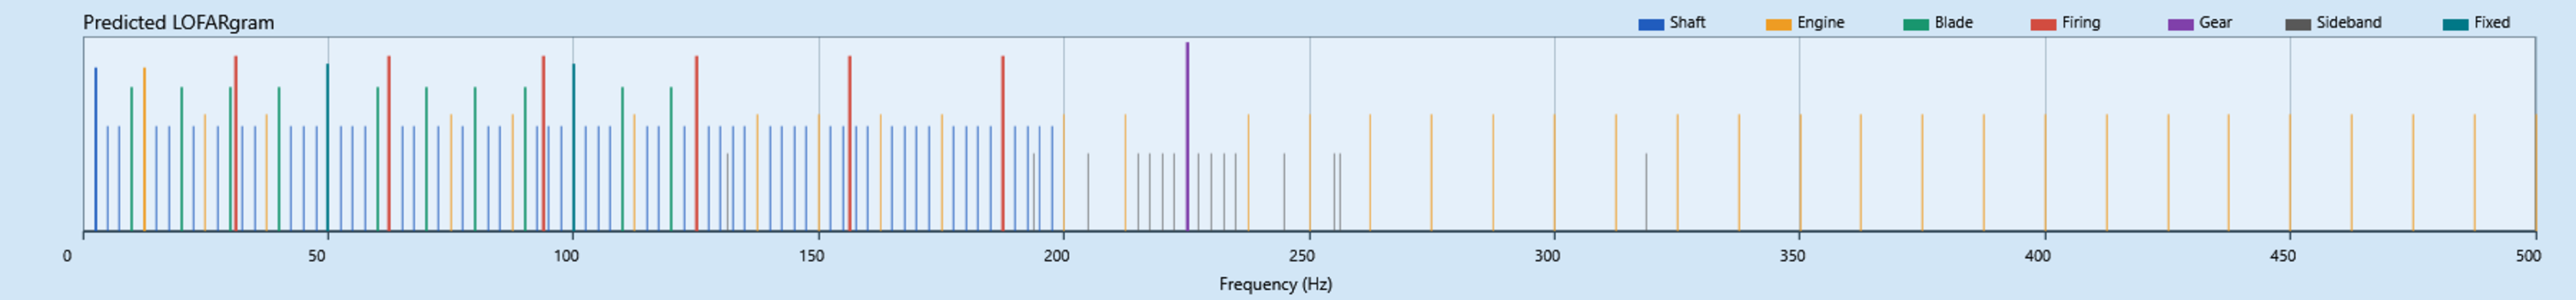
\includegraphics[width=\textwidth]{../img/actuals/lofar.pdf}
	\caption{All our data as a LOFARgram}
\end{figure}

\subsection{Recomended Workflow Using MACS}

Below is a recommended sequence for classifying an unknown contact. It applies equally to live capture and recorded file playback. Simply start capture or press [play] on a recording before beginning.
\subsubsection{Step 1 Clean up the signal}
\begin{compactenum}
    \item If own-ship or ambient noise is masking the target, designate a clean background recording as the noise reference and load it.
    \item Enable normalisation if tonals are weak against the noise floor. Adjust Scale until tonals are visible without the display saturating.
    \item If using a recorded file, apply the bandpass filter to isolate the frequency band of interest.
\end{compactenum}

\newcounter{myenum}
\setcounter{myenum}{\value{enumi}}

\subsubsection{Step 2 Identify tonals}
\begin{compactenum}
\setcounter{enumi}{\value{myenum}}
    \item On the LOFARgram (Panel A), note prominent vertical tonal lines.
    \item Use the harmonic cursor to test candidate fundamentals, place it on a suspected fundamental. Check whether the harmonic lines fall on other visible tonals. Do the same with sidebands.
    \item Zoom Fmin / Fmax to focus on dense tonal clusters.
    \item Mark confirmed tonals by selecting cursor mode and left-clicking on each line; right-click to clear.
\end{compactenum}

\setcounter{myenum}{\value{enumi}}

\subsubsection{Step 3 DEMON analysis}
\begin{compactenum}
\setcounter{enumi}{\value{myenum}}
    \item Open DEMON in Panel B.
    \item Set DEMON to a band with strong broadband noise (e.g. 500 - 5000 Hz).
    \item Identify the shaft rate peak (and / or diesel firing rate). Use the harmonic cursor to confirm the series.
    \item Note the shaft rate (SR) in rev/s.
\end{compactenum}

\setcounter{myenum}{\value{enumi}}

\subsubsection{Step 4 Cepstrum / ACF confirmation}
\begin{compactenum}
\setcounter{enumi}{\value{myenum}}  
    \item Switch Panel B to Cepstrum. Look for a quefrency peak confirming tonal spacing or shaft periodicity.
    \item Cross-check with ACF if needed.
\end{compactenum}

\setcounter{myenum}{\value{enumi}}

\subsubsection{Step 5 Record in database}
\begin{compactenum}
\setcounter{enumi}{\value{myenum}}
    \item In the right sidebar, enter a contact name in the \textbf{New Contact} field and click + Create with marked frequencies.
    \item Double-click the new contact to open the detail window.
    \item Enter propulsion type, blade count, shaft rate, speed, and any other known parameters. The app will auto-compute reduction factor and TPK.
    \item Add a note with the relevant recording filename for future reference (recording-to-contact linking is not yet available directly in the UI).
    \item \textbf{Save \& Close}
\end{compactenum}
\pagebreak